\section{Task Definition}
To collect vehicle data of the Fleet Management System (FMS) and provide IP-based access, a dedicated device has to be developed. It acts as a gateway (communication bridge) and connects the internal CAN-Bus to an Ethernet interface (LAN and wireless should be supported).


A general block diagram of the system is shown in \cref{fig:constellation_HW}.

\medskip
\begin{figure}[h!]
	\centering
	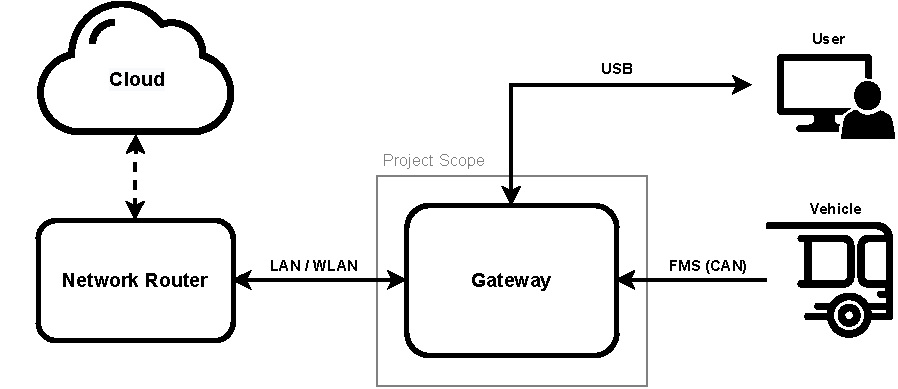
\includegraphics[width=9cm]{images/Block_Diagram}
	\caption{System Block Diagram}
	%\vspace{-2ex}
	%\caption*{\textbf{Source:} Original task definition}
	\label{fig:constellation_HW}
\end{figure}

FMS-Packages are received by the gateway and then get redirected to a local server application, running on the vehicles on-board network router.
Further, the information can be transmitted over the internet to a cloud-based system.

\begin{itemize}
	\item bla 1
	\item bla 2
	\item bla 3
\end{itemize}

Various use cases were defined in \cref{sec:use_cases}.